\documentclass[a4paper,11pt]{article}
\usepackage{polski}
\usepackage[utf8]{inputenc}
\usepackage{enumerate}
\usepackage{mathtools}
\usepackage{amsmath}
\usepackage{graphicx} 
\author{Filip Chodorowski}
\title{Sprawozdanie z laboratorium nr 7\\
„Złożoność obliczeniowa algorytmów w drzewie”}
\frenchspacing
\begin{document}
\maketitle
\tableofcontents
\section{Założenia zadania}
Zadanie polegało na zaimplementowaniu struktury drzewa binarnego i drzewa czerwono-czarnego z algorytmami dodawania i wyszukiwania elementów.
\newpage
\section{Zaimplementowane struktury}
\subsection{Drzewo binarne}
Drzewo binarne posiada co najwyżej 2 kolejne węzły. Jest strukturą niezbalansowaną tzn. wysokość drzewa może być dwukrotnie większa niż wysokość minimalna. Optymistyczna teoretyczna klasa złożoności podstawowych operacji:
$O(\log_2 n) 
$
W najgorszym przypadku drzewo binarne jest traktowane jak lista i złożoność podstawowych operacji wynosi wtedy:
$O(n) 
$
\subsection{Drzewo czerwono-czarne}
Drzewo czerwono-czarne jest odmianą drzewa binarnego, z tego powodu każdy węzeł posiada co najwyżej 2 kolejne. Jest strukturą zbalansowaną tzn. wysokość drzewa nie może być dwukrotnie większa niż wysokość minimalna. Ostatnie węzły są liściami, które wskazują adres węzła strażnika.Teoretyczna klasa złożoności podstawowych operacji:
$O(\log_2 n)
$
Nie ma przypadku pesymistycznego, ponieważ drzewo jest zbalansowane.
\newpage
\section{Wyniki}
\subsection{Porównanie dodawania elementów dla drzewa binarnego i drzewa czerwono-czarnego}
\begin{center}
\begin{figure}[h!]
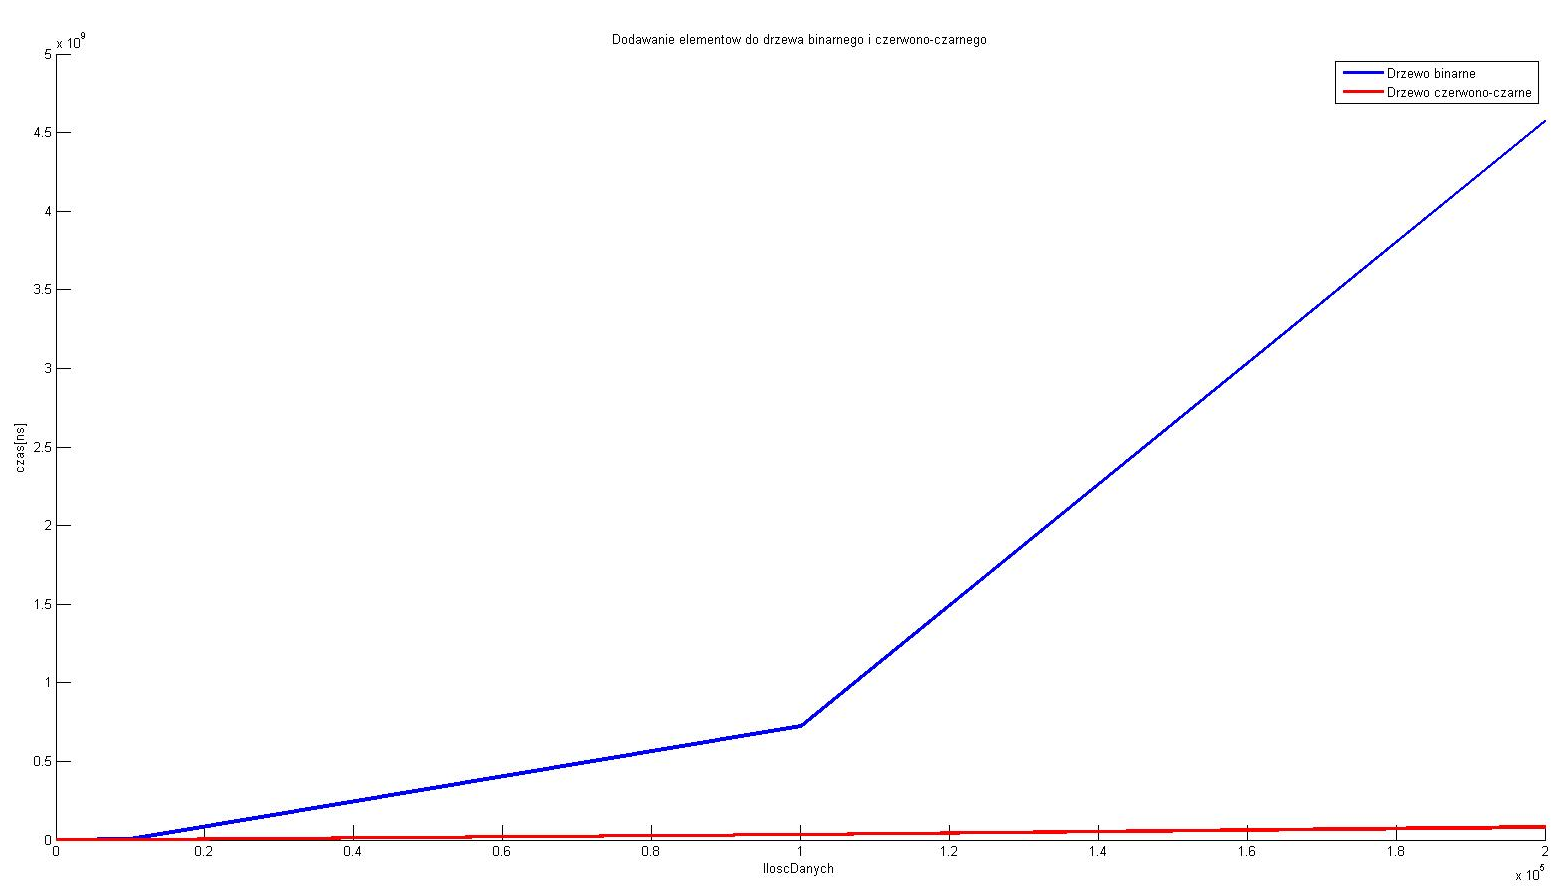
\includegraphics[width=12.5cm,height=10cm]{Wykresy2/DodawanieElementow}
%%\caption{Tu umieszczasz opis}
\label{fig:obrazek Wykresy2/DodawanieElementow}
\end{figure}
\end{center}
Drzewo binarne dodaje elementy szybciej dla rozmiaru 100,powyżej rozmiaru 100 drzewo czerwono-czarne jest szybsze, dla 200 000 elementów jest to różnica 100 razy i tendencja nadal rośnie. W obydwu drzewach elementy o takiej samej wartości są umieszczane w kolejnym niższym węźle. W drzewie binarnym struktura nie jest balansowana, co powoduje przy większych danych złożoność:
$O(n) 
$ 
\newpage
\subsection{Porównanie wyszukiwania wszystkich elementów drzewa dla drzewa binarnego i czerwono-czarnego}
\begin{center}
\begin{figure}[h!]
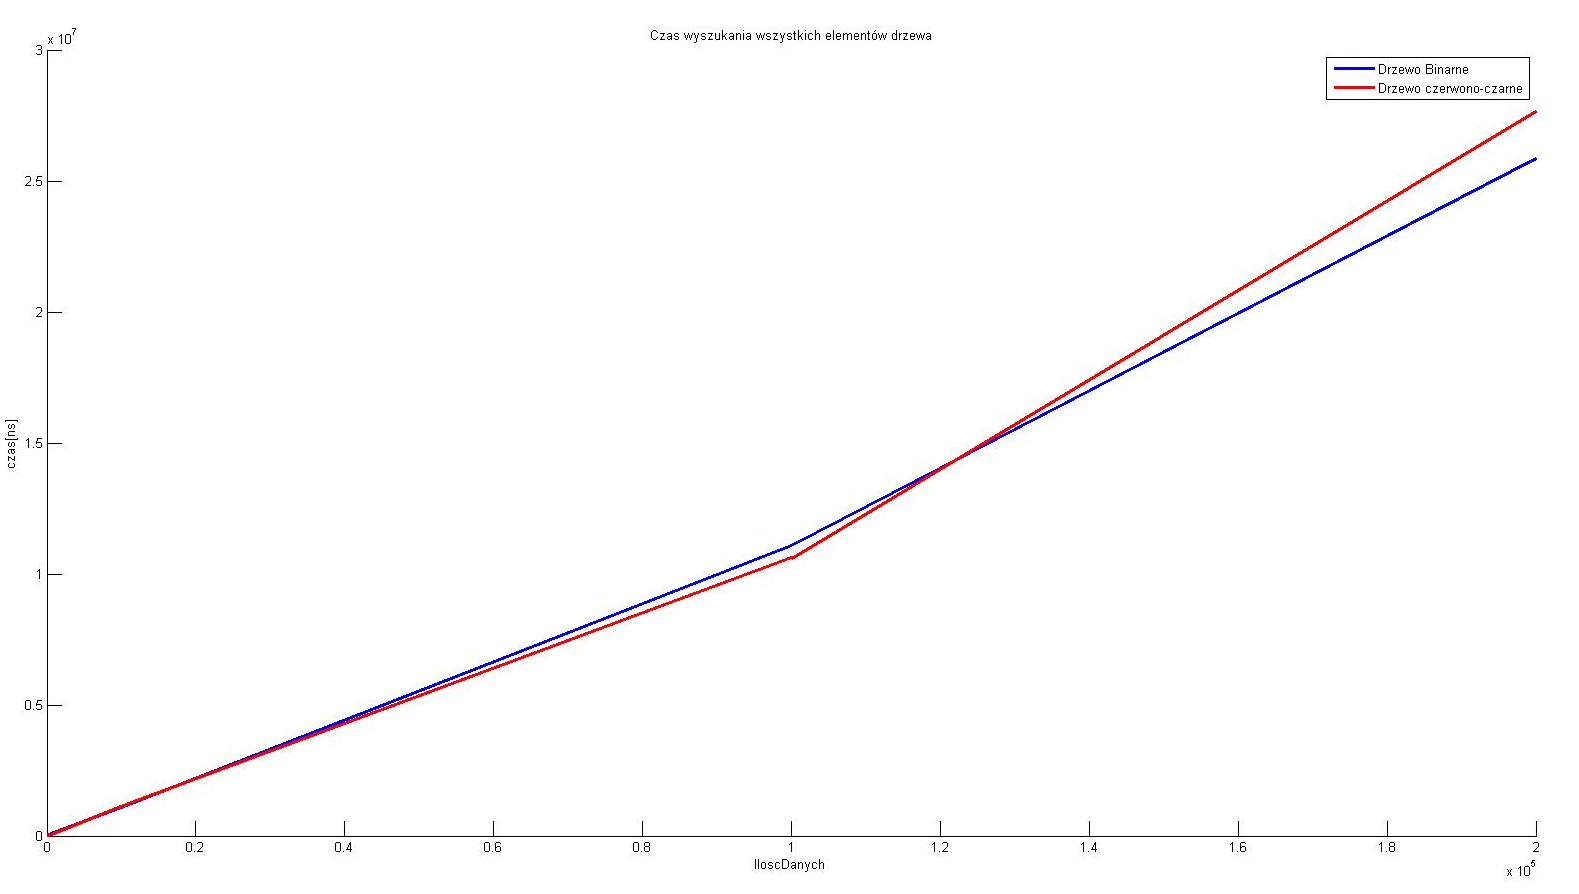
\includegraphics[width=12.5cm,height=10cm]{Wykresy2/WszystkieElementyWyszukaj}
%%\caption{Tu umieszczasz opis}
\label{fig:obrazek Wykresy2/WszystkieElementyWyszukaj}
\end{figure}
\end{center}
Czas wyszukania wszystkich elementów obydwu drzew jest tego samego rzędu. Wynika to z powtarzających się elementów w strukturach. Chociaż drzewo binarne nie jest zbalansowane to w tym konkretnym przypadku, odrzuca podczas wyszukiwania bardzo wiele elementów powtarzających się.
\newpage
\subsection{Porównanie wyszukiwania elementu nieznajdującego się w drzewach}
\begin{center}
\begin{figure}[h!]
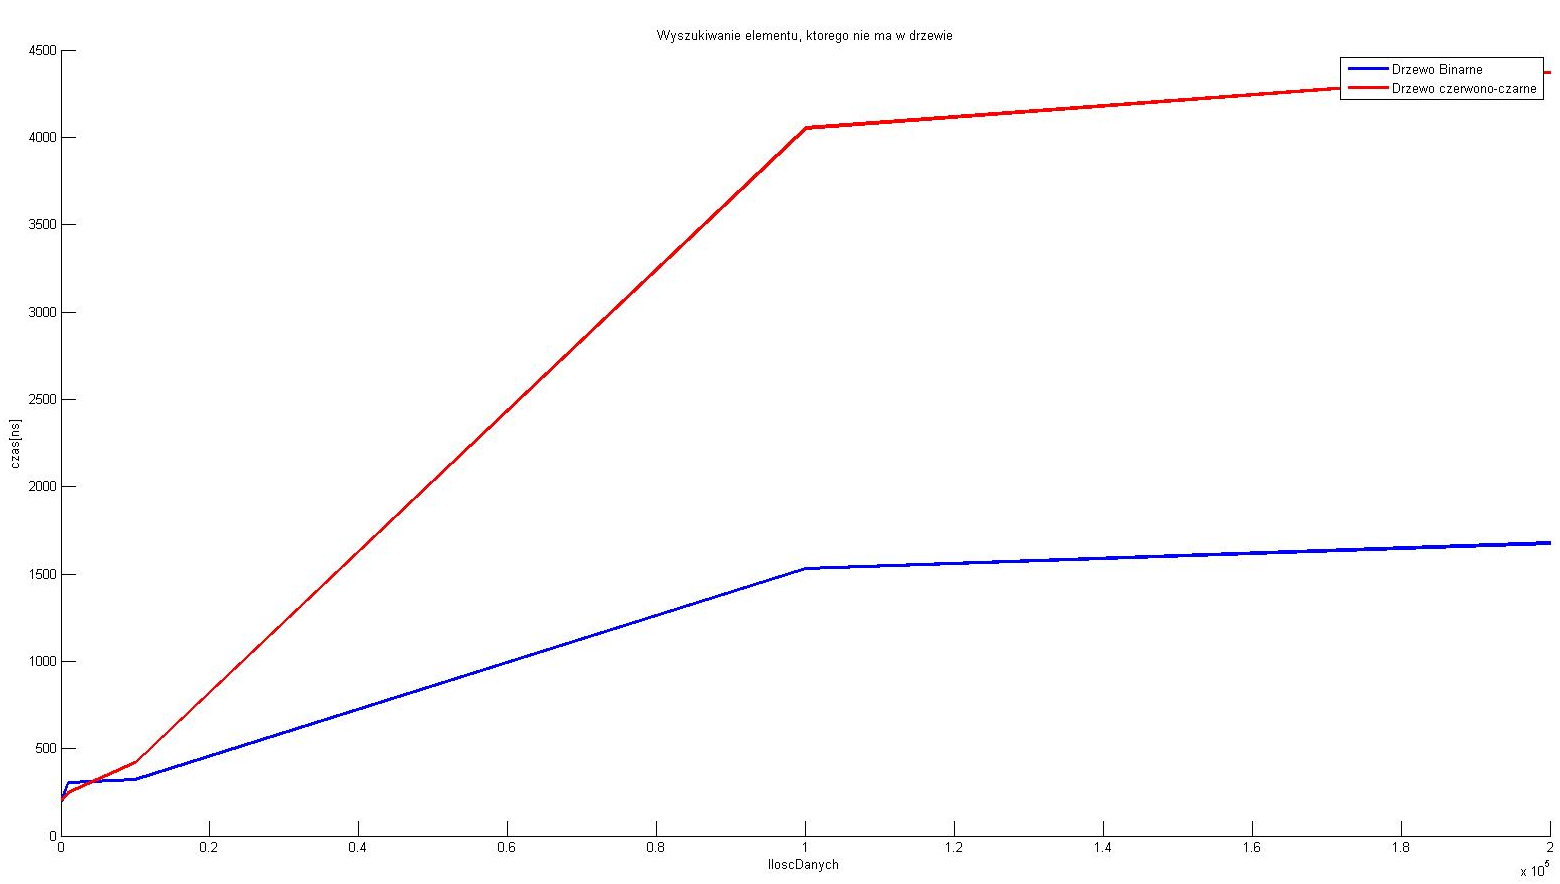
\includegraphics[width=12.5cm,height=10cm]{Wykresy2/NieIstniejacy}
%%\caption{Tu umieszczasz opis}
\end{figure}
\end{center}
Czas wyszukiwania nieistniejącego elementu w drzewie jest porównywalny dla. Dla drzewa binarnego czas wykonywania zależy od wyszukiwanego elementu, a dla drzewa czerwono-czarnego nie.
Złożoność wyszukiwania drzewa czerwono-czarnego:
$O(\log_2 n)
$
\\
Złożoność wyszukiwania drzewa binarnego:
Od
$O(\log_2 n)
$
do
$O(n) 
$ 

\newpage
\section{Wnioski}
\begin{itemize}
%\ldots
\item Drzewo czerwono-czarne ma stałą złożoność podstawowych operacji wynoszącą:
$O(\log_2 n)
$
\item Nowe elementy o tej samej wartości w drzewie binarnym(jeśli muszą być umieszczane) lepiej umieszczać w wyższych wierzchołkach, bo inaczej trzeba wykonać dodatkowe operacje przejścia na dół struktury.
\item drzewo czerwono-czarne $>$ binarne, chyba że mamy wcześniej posortowane elementy, wtedy można wykorzystać binarne bez obawy o złożoność $O(n) 
$ 
\end{itemize}
\end{document}